
\section{Introduction}

The \SoftwareName (Multi-Criteria Decision Analysis MEthods Assessment through SimUlation REsearch) software includes a game module using the Unity game engine and a library created in the Matlab/Octave environment. The game module can be controlled using commands in which data is saved in XML format (fig.~\ref{Fig:architecture}). Responsible for visualizing the game board and controlling its course. By default, the game is configured to listen on port 55001. The default address (127.0.0.1) allows you to connect to the game only from the computer on which it is installed (however, this can be changed).

The library is intended to facilitate the creation of software in Matlab/Octave intended for testing decision support methods. Contains methods for preparing and formatting commands to be sent to the game. It also allows you to decode the answers received from the game. An additional option of the library is the conversion of tables to the tabular Latex environment format and a format that allows them to be read by the tikz package's charting module.

\begin{figure}
\begin{tikzpicture}
\node[rectangle,draw,minimum width = 3.5cm,minimum height = 1.5cm,label=above:{Player}] (r) at (-2.5,4.5) {Matlab/Octave};
\node[anchor=center,inner sep=0,label=above:{Game}] (game) at (4,4.5) {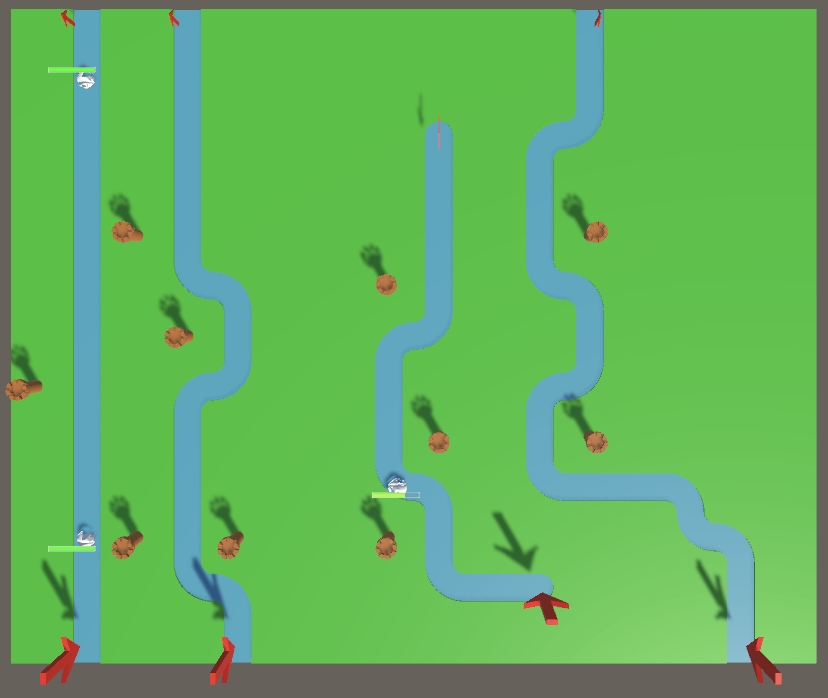
\includegraphics[width=3cm]{images/game.png}} ;
\node[anchor=center,inner sep=0, label=below:{Reports}] (tabaular) at (-2.5,1) {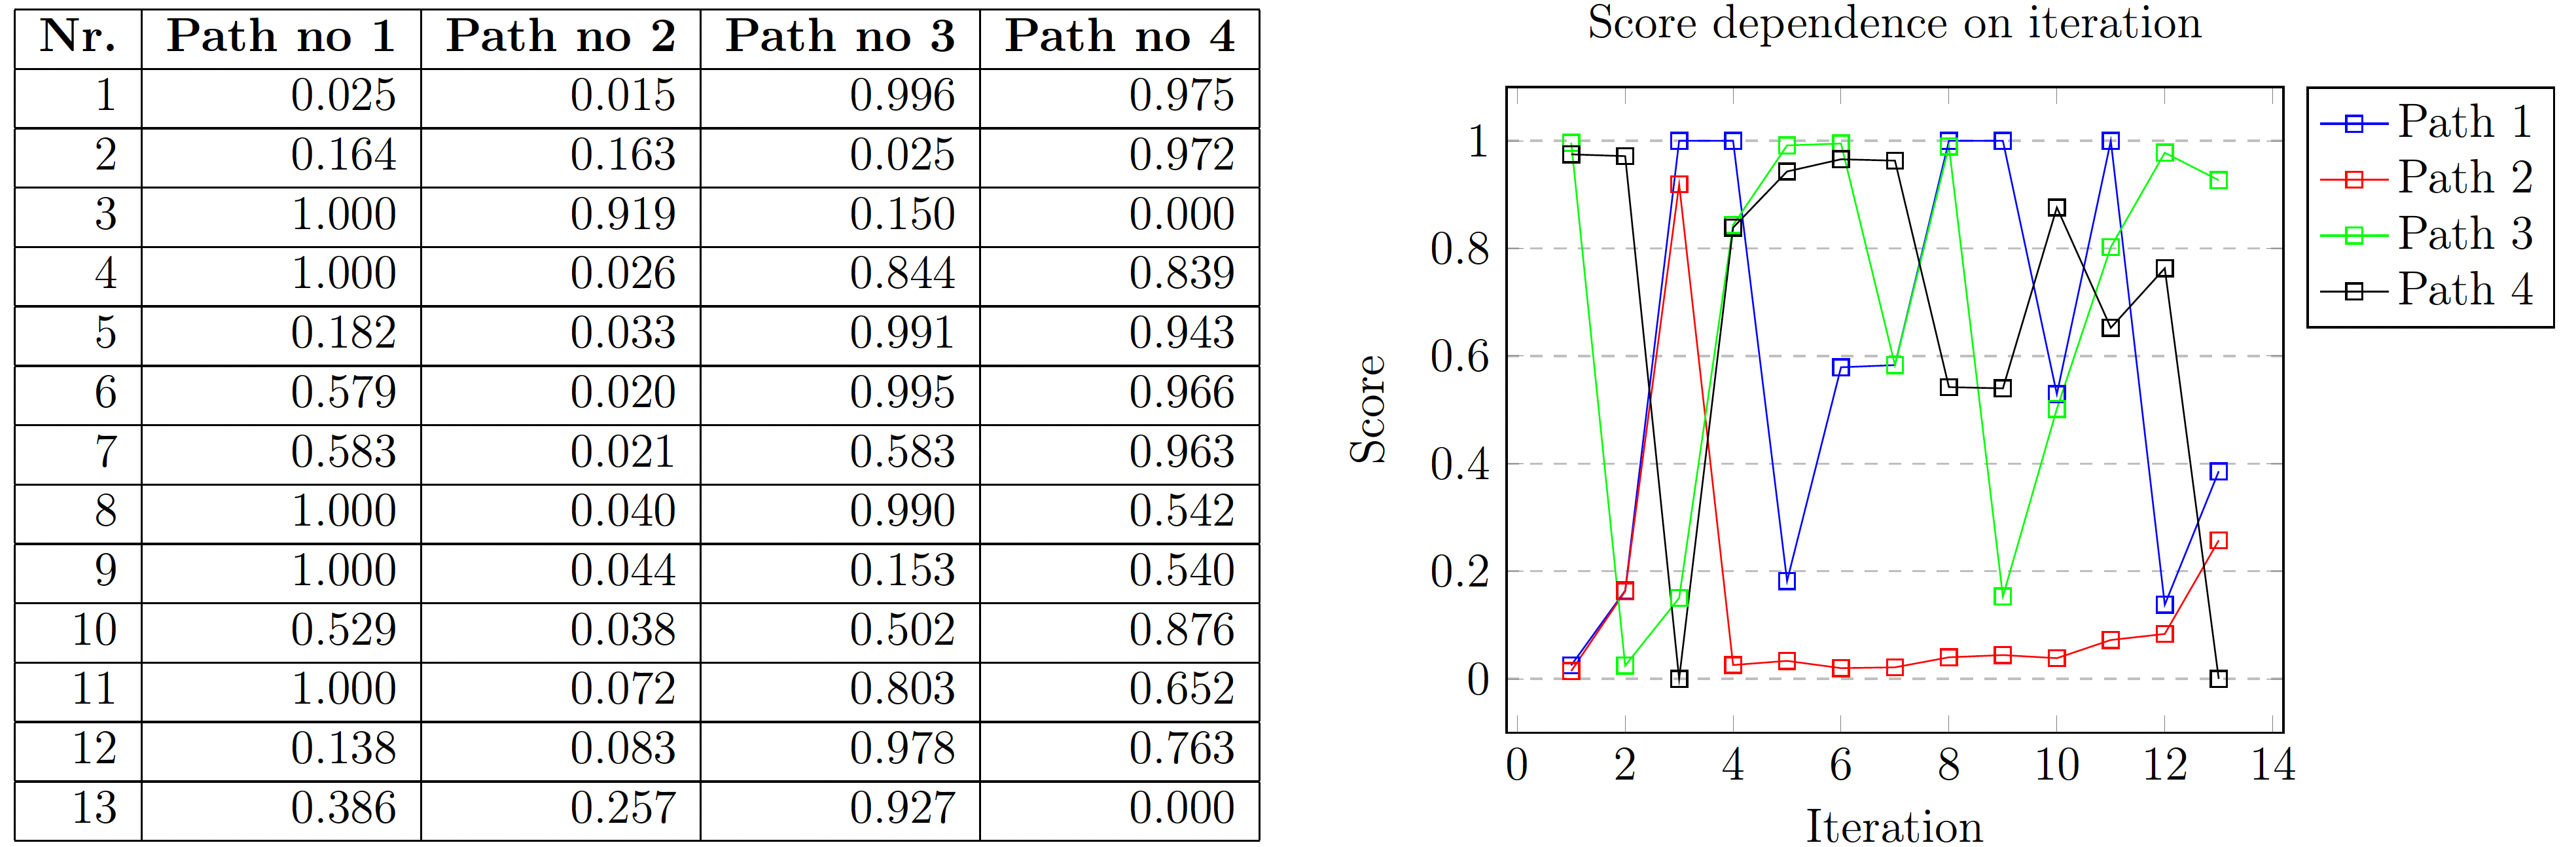
\includegraphics[height=2.5cm]{images/latexReports.png}};
\draw[oneArrowinverseStyle] (r.east) + (0,-0.1) -- ++(3.3,-0.1) node[midway,below]{Answer};
\draw[oneArrowStyle] (r.east) + (0,0.1) -- ++(3.3,0.1) node[midway,above]{Command};
\draw[oneArrowStyle] (r) -- (tabaular);

\end{tikzpicture}

\caption{System architecture}
\label{Fig:architecture}
\end{figure}